% ------------------------------------------------------------------------
% ------------------------------------------------------------------------
% ------------------------------------------------------------------------
%                                Capítulo 4
% ------------------------------------------------------------------------
% ------------------------------------------------------------------------
% ------------------------------------------------------------------------

\chapter{SIMULACIONES Y RESULTADOS}

En esta sección se presentan los resultados obtenidos a partir del método propuesto para la clasificación de objetos basado en medidas medidas cuadráticas codificadas y su comparación con esquemas de clasificación del estado del arte.

\section{CONJUNTO DE DATOS}

Durante el desarrollo de este trabajo, no se encontraron conjuntos de datos públicos enfocados en la clasificación de medidas cuadráticas. Debido a esto, se decidió simular la propagación de las medidas usando conjuntos de datos tradicionales. Para este fin se usaron imágenes de los conjuntos de datos MNIST \myfootcite{deng2012mnist} y Fashion-MNIST \myfootcite{xiao2017fashion}. Por un lado, la Figura \ref{fig:conjunto_datos} muestra un ejemplo de las imágenes presentes en los conjuntos de datos usados. Por otro lado, la Tabla \ref{tab:conjunto_datos} muestra la división de datos en entrenamiento, validación y prueba. Cada imagen fue escalada en el rango de $[-\pi, \pi]$ y usada como información de fase de la forma $\mathbf{z}=e^{j\mathrm{ang}(\mathbf{z})}$.

\begin{figure}[!h]
    \centering
    \caption{Ejemplo de las imágenes presentes en los conjuntos de datos MNIST y Fashion-MNIST.}
    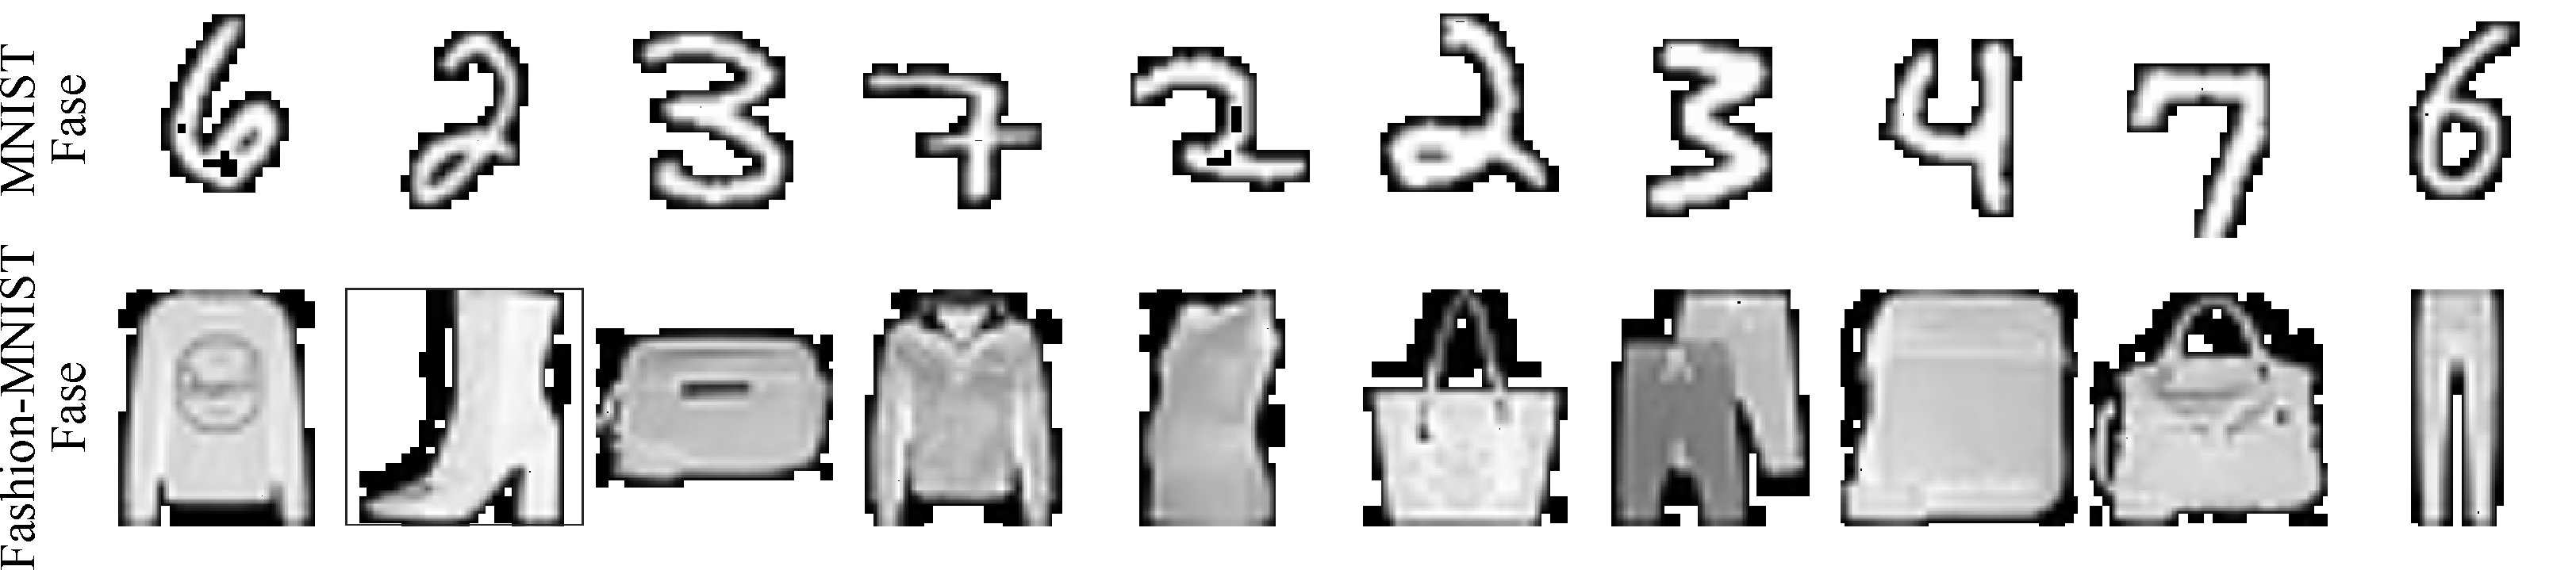
\includegraphics[width=\linewidth]{images/resultados/datasets.pdf}
    \label{fig:conjunto_datos}
\end{figure}


% Please add the following required packages to your document preamble:
% \usepackage{graphicx}
\begin{table}[!h]
\caption{Resumen de la división de los conjuntos de datos usados para evaluar el método propuesto.}
\centering\scalebox{0.9}{
\resizebox{\textwidth}{!}{%
\begin{tabular}{|c|c|c|c|c|}
\hline
\textbf{Conjunto de datos} & \textbf{Entrenamiento} & \textbf{Validación} & \textbf{Prueba} & \textbf{Total} \\ \hline
MNIST                      & 54000                  & 6000                & 10000           & 70000          \\ \hline
Fashion-MNIST              & 54000                  & 6000                & 10000           & 70000          \\ \hline
\end{tabular}%
}}
\label{tab:conjunto_datos}
\end{table}

\section{MÉTRICAS}
La calidad de la inicialización y la precisión de la clasificación en sistemas de difracción basados en medidas cuadráticas codificadas, se mide a través de las siguientes métricas.
\subsection{Métricas para evaluar la inicialización.}

A continuación, se describen las métricas usadas para evaluar la estimación inicial $\hat{\mathbf{z}}$ respecto a la imagen de referencia $\mathbf{z}$.
\begin{itemize}
    \item Medida del índice de similitud estructural (SSIM):
    
    \begin{equation}
        %\nonumber
        \mathrm{SSIM}(\mathbf{z}, \tilde{\mathbf{z}}) = \frac{2(\mu_{\mathbf{z}}\mu_{\tilde{\mathbf{z}}} + C_1) + (2\sigma_{\mathbf{z}\tilde{\mathbf{z}}} + C_2)}{(\mu_{\mathbf{z}} + \mu_{\tilde{\mathbf{z}}} + C_1)(\sigma_{\mathbf{z}}\sigma_{\tilde{\mathbf{z}}} + C_1)},
        \label{eq:SSIM}
    \end{equation}
    
    donde $(\mu_{\mathbf{z}}, \sigma_{{\mathbf{z}}})$ y $(\mu_{\tilde{\mathbf{z}}}, \sigma_{\tilde{\mathbf{z}}})$ representan la media y la varianza de ${\mathbf{z}}$ y $\tilde{\mathbf{z}}$ respectivamente, además $\sigma_{\mathbf{z}\tilde{\mathbf{z}}}$ es la covarianza entre ellos. Por último, $C_1 = (k_1L)^2$ y $C_2 = (k_2L)^2$ son dos constantes para prevenir división por cero y $k_1 = 0.01$ y $k_2 = 0.03$. Esta métrica tiene valores en el rango de $[0, 1]$, es decir, a mayor valor, mejor es la estimación.
    
    \item Relación de señal a ruido máxima (PSNR):
    \begin{equation}
        %\nonumber
        \mathrm{PSNR}(\mathbf{z}, \tilde{\mathbf{z}})=10 \cdot \log_{10}\left(\frac{\mathrm{MAX}^{2}}{\mathrm{MSE}(\mathbf{z}, \tilde{\mathbf{z}})}\right),
        \label{eq:PSNR}
    \end{equation}
    donde $\mathrm{MAX}(\cdot)$ es el rango dinámico de la imagen y $\mathrm{MSE}(\cdot)$ es el error cuadrático medio entre la imagen original y la estimación. Esta métrica tiene valores en el rango de $[0, \infty)$, es decir, a mayor valor, mejor es la estimación.
    
    \item Error cuadrático medio (MSE):
    
    \begin{equation}
        %\nonumber
        \mathrm{MSE}(\mathbf{z}, \tilde{\mathbf{z}}) = \frac{1}{n} \Vert \mathbf{z} - \tilde{\mathbf{z}}\Vert_2^2.
        \label{eq:MSE}
    \end{equation}
    
    Esta métrica tiene valores en el rango de $[0, \infty)$, es decir, a menor valor, mejor es la estimación.

    \item Error relativo (RE): 
    \begin{equation}
        %\nonumber
        \mathrm{RE}(\mathbf{z}, \tilde{\mathbf{z}}) = \frac{ \mathrm{dist}(\mathbf{z}, \hat{\mathbf{z}})}{\Vert \mathbf{z} \Vert_2}.
        \label{eq:RE}
    \end{equation}
    
    Esta métrica tiene valores en el rango de $[0, \infty)$, donde a menor valor, mejor es la estimación.
\end{itemize}
\subsection{Métricas para evaluar la clasificación.}
Las métricas usadas para evaluar la clasificación se presentan a continuación, donde los valores a calcular dependen de los verdaderos positivos $TP$, verdaderos negativos $TN$, falsos positivos $FP$, y falsos negativos $FN$, asociados a la clase de cada ejemplo del conjunto de datos.


\begin{itemize}
    \item Exactitud: esta medida corresponde a la proporción de predicciones predichas correctamente,

    \begin{equation}
        \mathrm{Exactitud}= \frac{TP+TN}{TP+TN+FP+FN}.
        \label{eq:acc}
    \end{equation}


    \item Precisión: esta medida es la proporción de ejemplos pertenecientes a una clase que fueron correctamente predichos en dicha clase,
    
        \begin{equation}
            \mathrm{Precision} = \frac{TP}{TP+FP}.
            \label{eq:pre}
        \end{equation}
        
    \item Exhaustividad: esta medida es la proporción entre las predicciones que fueron correctamente clasificadas en una clase sobre los ejemplos que pertenecían a esa clase,
    
    \begin{equation}
        \mathrm{Exhaustividad}= \frac{TP}{TP+FN}.
        \label{eq:re}
    \end{equation}

    \item Métrica-F1: esta medida está diseñada para ponderar de manera equilibrada entre las métricas de precisión (\ref{eq:pre}) y exhaustividad (\ref{eq:re}),
    
    \begin{equation}
        \mathrm{F1} = \frac{2\cdot\mathrm{Precision}\cdot\mathrm{Exhaustividad}}{\mathrm{Precision}+\mathrm{Exhaustividad}}.
        \label{eq:f1}
    \end{equation}

\end{itemize}

\section{EXPERIMENTOS}

% \subsection{Métodos de Comparación}

% \begin{itemize}
%     \item Comparación estimación inicial.
    
%     Estimar el campo óptico inicial es una tarea ampliamente estudiada en el estado del arte de recuperación de la fase. Específicamente resaltan métodos tales como el propuesto \myfootcite{Morales:22}, \textit{orthogonality-promoting initialization} (OPI) \myfootcite{wang2017solving}, \textit{weighted maximal correlation initialization} (WMCI) \myfootcite{wang2018phase}, y \textit{filtered spectral initialization} (FSI) \myfootcite{jerez2020fast}. Estos métodos de estimación inicial son usados como etapa inicial por algoritmos de reconstrucción tales como TWF, TAF y RAF.
    
    
%     \item Comparación clasificación.
    
%     Para comparar el método propuesto se encontró que el esquema tradicional de clasificación sobre medidas cuadráticas se realiza como se muestra en la Figura \ref{fig:esquema_entrenamiento_tradicional}
    
%     \begin{minipage}[!h]{\linewidth}
      
%       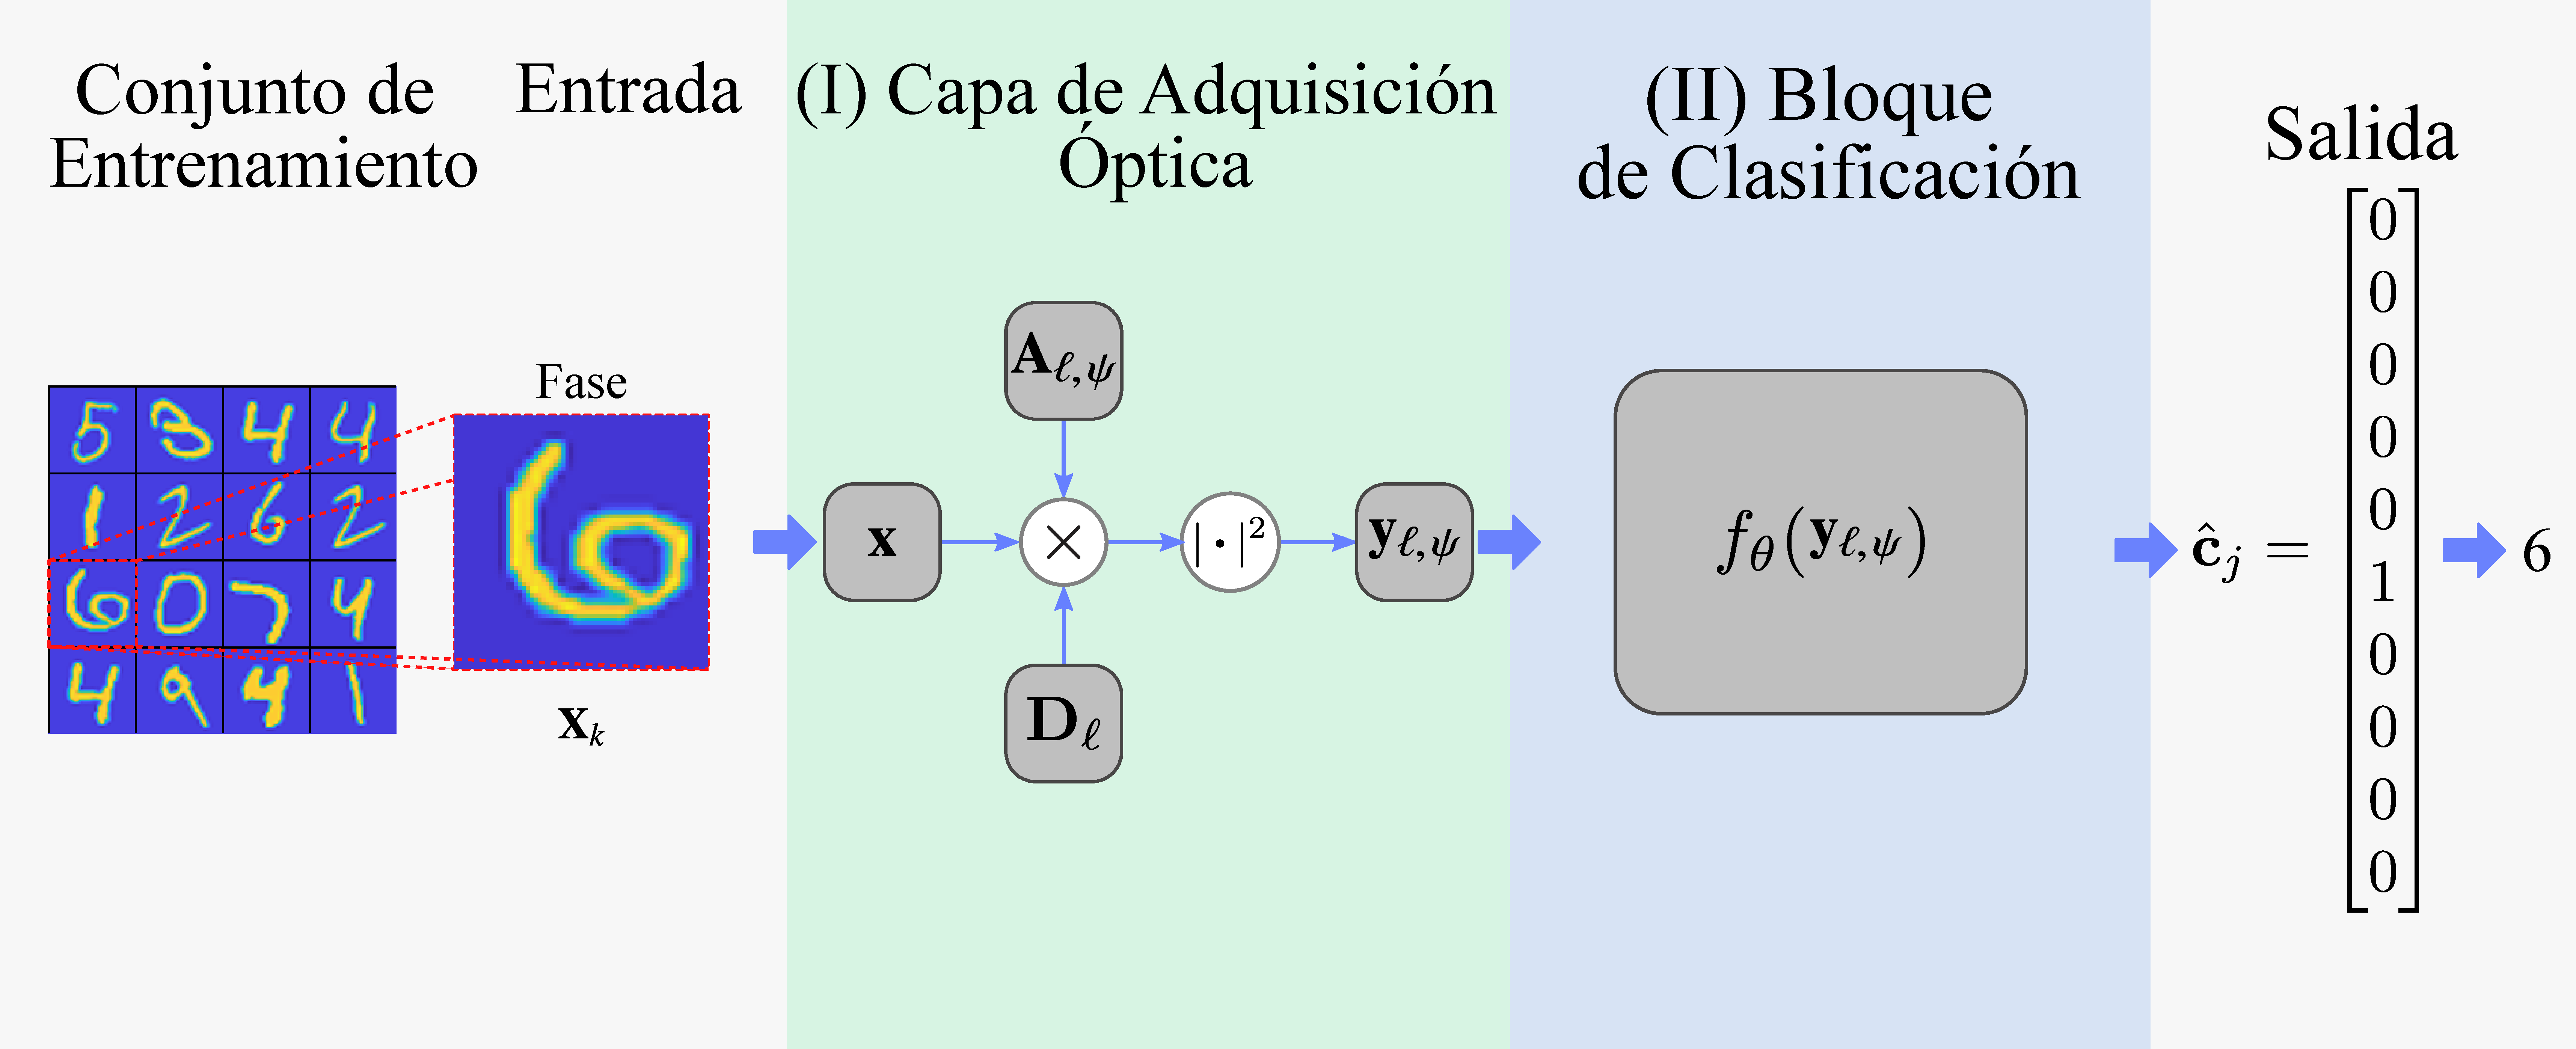
\includegraphics[width=\linewidth]{images/metodología/esquema_entrenamiento_tradicional.pdf}
%       \captionof{figure}{Esquema de clasificación usado en el estado del arte.}
%         \label{fig:esquema_entrenamiento_tradicional}
%     \end{minipage}
    
%     En el esquema tradicional no se realiza una modulación del campo óptico, por lo tanto para la comparación con el estado del arte la codificación corresponde a $\mathbf{D}_\ell = 1$.
    
%     Adicionalmente se realizó la comparación haciendo uso del operador inverso de la propagación del campo óptico $\mathcal{P}_{\ell, \psi}:\mathbb{C}^n\rightarrow \mathbb{C}^n$ para estimar $\hat{\mathbf{x}}$ \myfootcite{katkovnik2017computational},
    
%     \begin{equation}
%         \hat{\mathbf{x}}= \frac{1}{L}\sum_{\ell=1}^{ L} \mathcal{P}_{\ell, \psi}(\mathbf{y}_{\ell, \psi}).
%         \label{eq:back_propagation}
%     \end{equation}
% \end{itemize}

\subsection{Configuración experimental.}

En esta subsección, se presentan los parámetros de simulación utilizados para el modelo de propagación, la etapa de inicialización y la red neuronal de clasificación. Todos los experimentos realizados en este trabajo fueron implementados en \textit{Python 3.9} usando la herramienta \textit{Tensorflow 2.4.1}  \myfootcite{tensorflow2015-whitepaper}. Los experimentos se ejecutaron sobre un computador con GPU Nvidia 3090 RTX con 64 Gb de memoria RAM y CPU Intel(R) Xeon(R) W-3223 CPU @ 3.50GHz. El código usado para los experimentos de este trabajo puede ser consultado de manera pública en \footnote{\href{https://github.com/David-Morales-Norato/code_undergrad_thesis}{https://github.com/David-Morales-Norato/code\_undergrad\_thesis}}. En relación con los parámetros de propagación,  la Tabla \ref{tab:parameters} presenta los parámetros ópticos fijados para calcular la matriz $\mathbf{A}_{\ell,\psi}$ definida en \eqref{eq:phase_retrieval_problem} según cada campo de difracción. Estos parámetros permiten simular la adquisición de las medidas cuadráticas codificadas a lo largo de cada campo de difracción usando la capa de adquisición óptica. En la etapa de inicialización, el filtro $\mathbf{G} \in \mathbb{C}^{g\times g}$ entrenable fue fijado a un tamaño de kernel $g=5$ y un número de iteraciones $T=10$. La estimación del campo óptico inicial es una tarea ampliamente estudiada en el estado del arte de recuperación de la fase. Específicamente, se destacan métodos de inicialización, tales como \textit{orthogonality-promoting initialization} (OPI) \myfootcite{wang2017solving}, \textit{weighted maximal correlation initialization} (WMCI) \myfootcite{wang2018phase}, y FSI \myfootcite{jerez2020fast}. Cabe señalar que, estos métodos de inicialización fueron usados para comparar la inicialización propuesta LFSI, donde se comparó la robustez al ruido, el número de iteraciones ${T}$ y el número de proyecciones ${L}$ requeridas para lograr una estimación apropiada. 

Finalmente, para realizar la clasificación se usaron las arquitecturas MobilNetV2 \myfootcite{mobilnetv2}, InceptionV3 \myfootcite{inceptionv3} y Xception \myfootcite{xception}, las cuales fueron entrenadas usando una tasa de aprendizaje de $1\times 10^{-3}$ con el algoritmo de optimización Adam a partir de $\mathcal{E}=100$ épocas para entrenar los conjuntos de datos MNIST y Fashion-MNIST. Para comparar el esquema de clasificación propuesto se implementó el esquema de clasificación tradicional \myfootcite{kim2018deep}$^,$\myfootcite{ ziletti2018insightful}, donde se realiza únicamente el proceso de simulación de las medidas cuadráticas sin el proceso de estimación del campo óptico. Asimismo, se empleó el método propuesto de filtrado espectral aprendido en las Figuras \ref{fig:results_mob}, \ref{fig:results_inc} y \ref{fig:results_xce}. Por otra parte, se reemplazó en la etapa de inicialización del esquema de clasificación propuesto, el algoritmo de inicialización LFSI por el modelo de propagación inverso (BPM, de sus siglas en inglés \textit{back-propagation matrix}) $\mathbf{A}_{\ell, \psi}^{-1}$ para obtener una estimación rápida del campo óptico inicial, como se presenta en las Figuras \ref{fig:results_mob}, \ref{fig:results_inc} y  \ref{fig:results_xce}. Esta estimación rápida está dada por 

\begin{equation}
    \hat{\mathbf{z}}= \frac{1}{L}\sum_{\ell=1}^{ L} \mathbf{A}_{\ell, \psi}^{-1}\mathbf{y}_{\ell, \psi}
    \label{eq:back_propagation}.
\end{equation}

Es importante señalar que, $\mathbf{z} \neq \mathbf{A}_{\ell, \psi}^{-1}\mathbf{y}_{\ell}$, debido a la pérdida de la información de fase que induce el operador de magnitud $\vert \cdot \vert$ presente en el modelo de propagación \eqref{eq:phase_retrieval_problem}.


% Por último, todos los experimentos realizados en este trabajo fueron implementados en \textit{Python 3.9} usando la herramienta \textit{Tensorflow 2.4.1}  \myfootcite{tensorflow2015-whitepaper}. Los experimentos se ejecutaron sobre un computador con GPU Nvidia 3090 RTX con 64 Gb de memoria RAM y CPU Intel(R) Xeon(R) W-3223 CPU @ 3.50GHz. El código usado para los experimentos de este trabajo puede ser consultado de manera pública en el siguiente enlace: \href{https://github.com/David-Morales-Norato/code_undergrad_thesis}{https://github.com/David-Morales-Norato/code\_undergrad\_thesis}

\begin{table}[!h]
\centering
\caption{ Parámetros de propagación usados para simular el modelo de propagación \eqref{eq:phase_retrieval_problem} para cada campo de difracción.}
\scalebox{0.9}{
\begin{tabular}{|l|r|r|c|}
\hline
\multicolumn{1}{|c|}{\textbf{Parámetros ópticos}} & \multicolumn{1}{c|}{\textbf{Campo cercano}} & \multicolumn{1}{c|}{\textbf{Campo medio}} & \textbf{Campo lejano} \\ \hline
Longitud de onda ($\lambda$) [nm]                    & 635                           & 635                            & -         \\ \hline
Distancia de propagación ($z$) [cm]         &    2.5                       & 7                              & -         \\ \hline
\end{tabular}}
\label{tab:parameters}
\end{table}


\subsection{Resultados de la inicialización.}


La Figura \ref{fig:results_initializations} muestra el desempeño en la métrica de RE del método de estimación inicial propuesto comparando con los algoritmos FSI, OPI y WMCI variando el número de iteraciones $T$ para los conjuntos de datos MNIST y Fashion-MNIST en los tres campos de difracción cercano, medio y lejano, donde se puede observar que el método propuesto logra superar los métodos tradicionales obteniendo una estimación inicial apropiada a partir de un número menor de iteraciones.

\begin{figure}[!h]
\centering
    \caption{Resumen del desempeño de la inicialización propuesta comparando con los métodos FSI, OPI, WMCI sobre la métrica de RE, variando el número de iteraciones del algoritmo para estimar imágenes de los conjuntos MNIST y Fashion-MNIST en los campos de difracción cercano, medio y lejano.}
    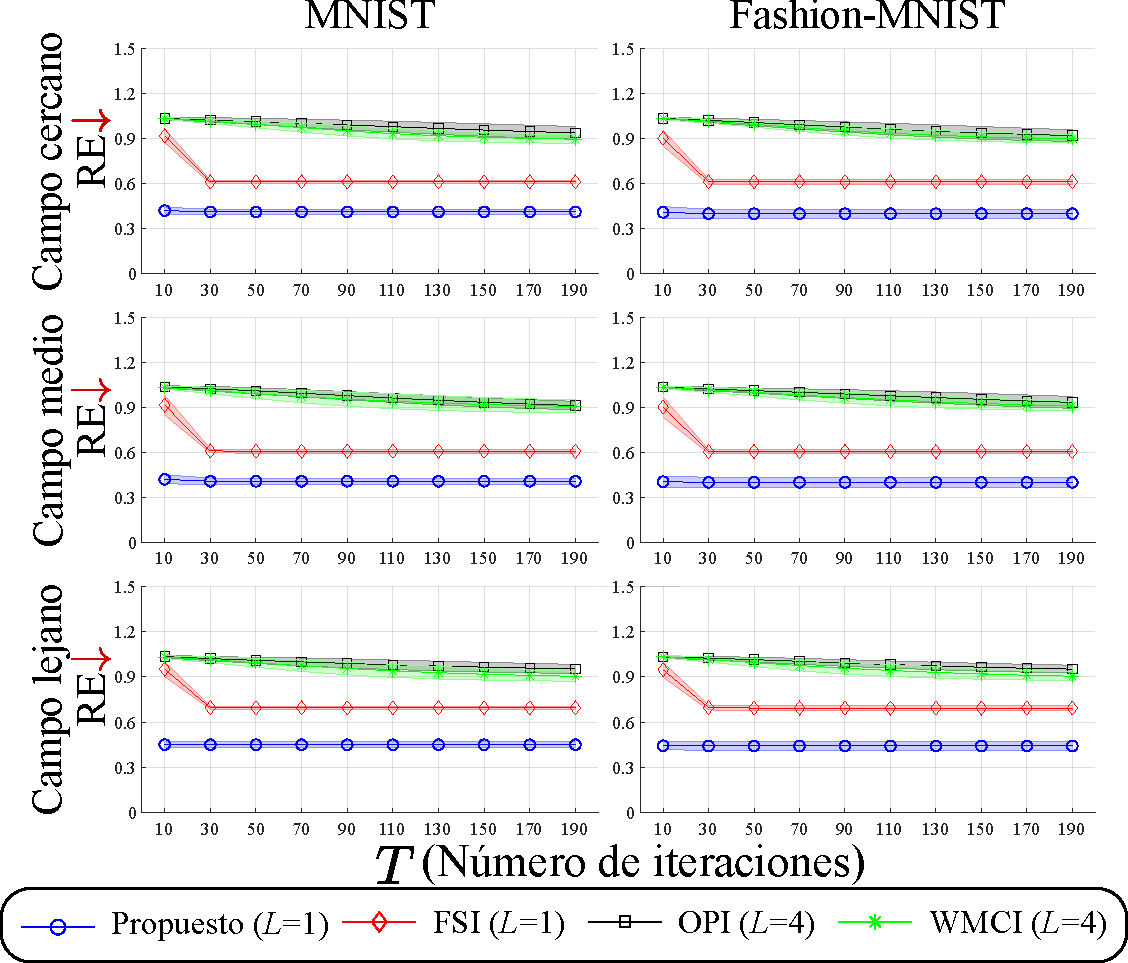
\includegraphics[width=0.85\linewidth]{images/resultados/results_initializations.pdf}
        \label{fig:results_initializations}
\end{figure}



La Figura \ref{fig:noisy_scenario} muestra la evaluación de la robustez del método frente al ruido. En este caso, se adicionó ruido aditivo gaussiano con $\mathrm{SNR} = 10, 15$ y $30$. Cabe resaltar que, el método propuesto muestra una mayor estabilidad al ruido comparando con los métodos de inicialización del estado del arte.

\begin{figure}[!h]
    \caption{Resumen del desempeño de la inicialización comparando con diferentes estrategias del estado del arte. Se varió el número de medidas $T$ para realizar la estimación y diferentes niveles de ruido afectando las medidas descritos por el SNR.}
    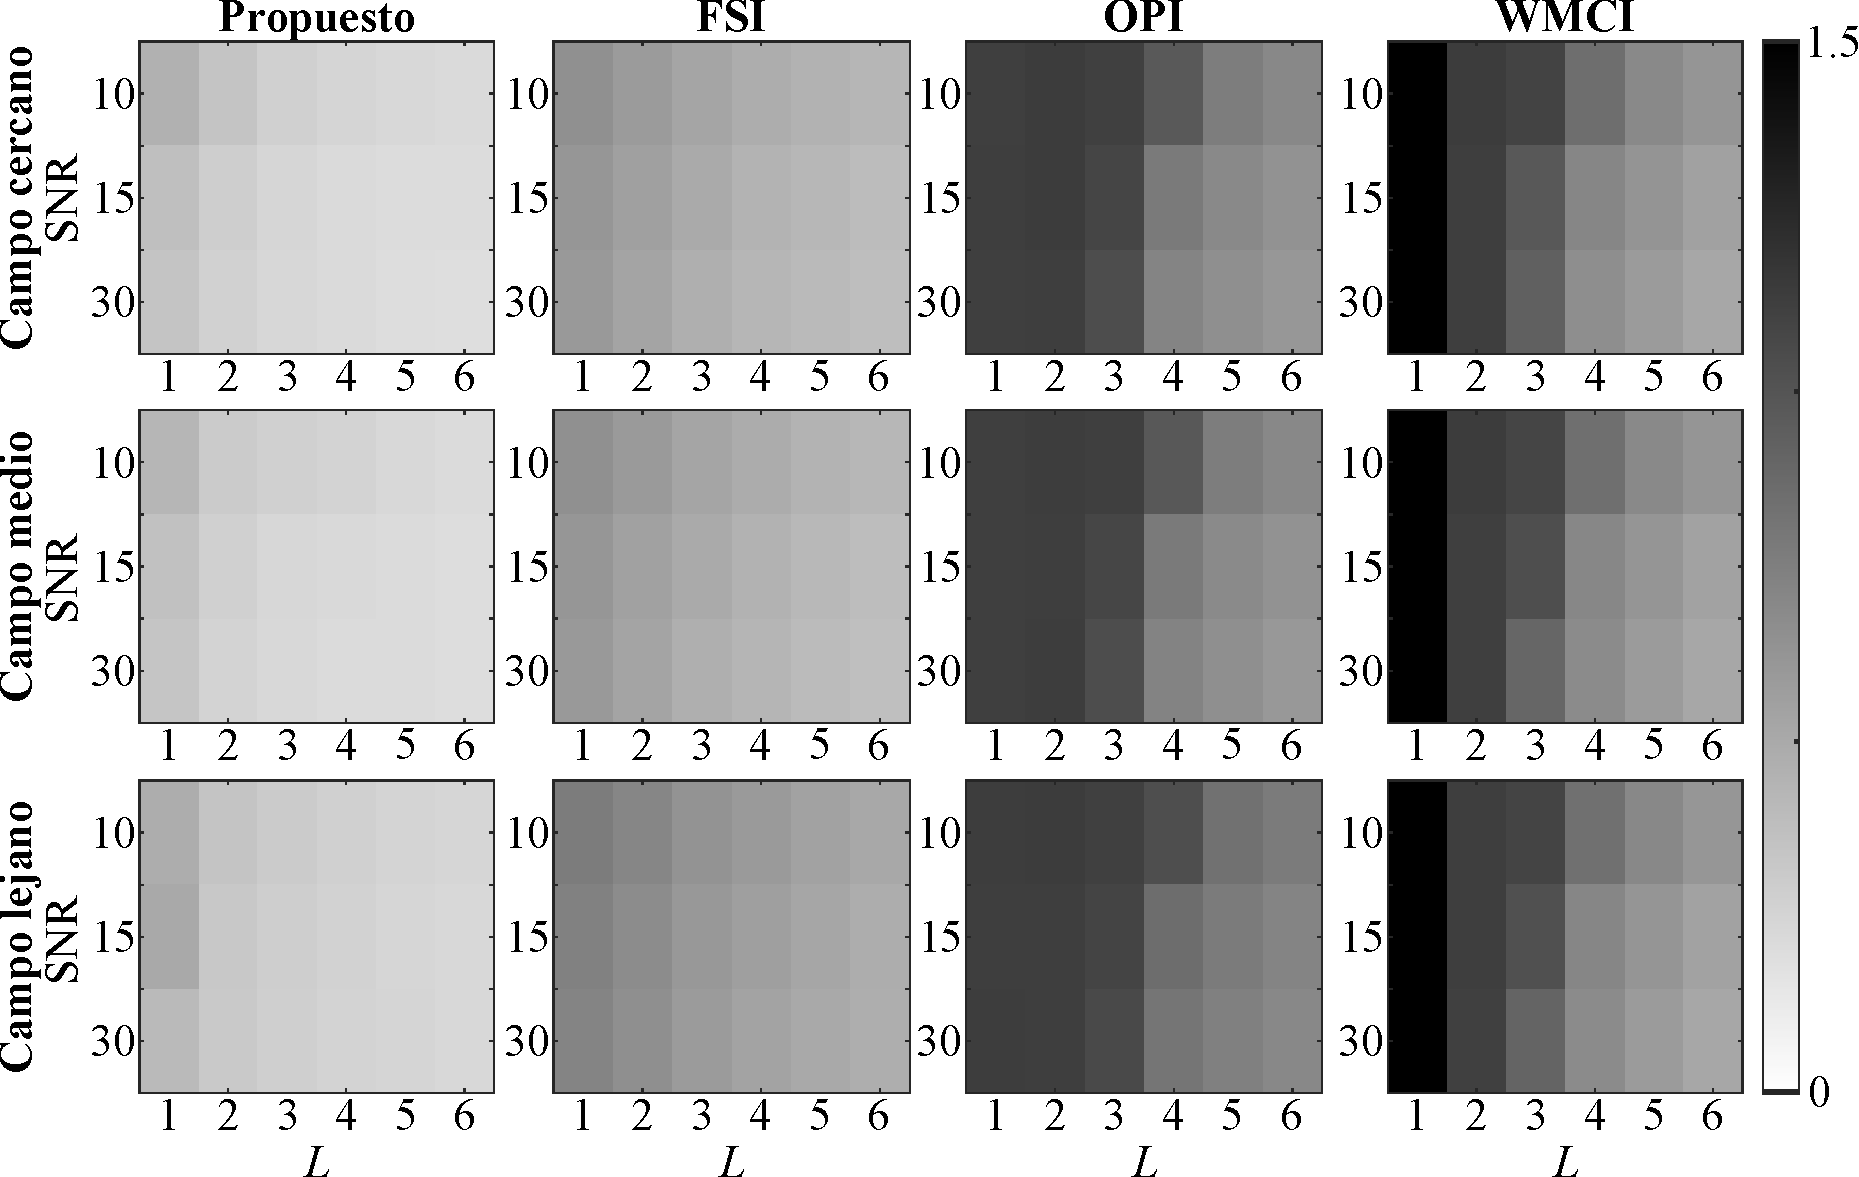
\includegraphics[width=1\linewidth]{images/resultados/Noisy_Initializations.pdf}
    \label{fig:noisy_scenario}
\end{figure}

Por último, la Figura \ref{fig:resultados_inicialización_sin_ruido} presenta los resultados visuales de la estimación del campo inicial para el conjunto de datos MNIST y Fashion-MNIST. Para comparar el método propuesto se implementaron los algoritmos FSI con $L = 1, T = 10$, FSI usando $L = 1, T=200$, OPI $L = 4, T=200$ y WMCI $L = 4, T=200$. Se puede observar que, el método propuesto logra aproximar el campo óptico en los tres campos de difracción simulados a un bajo número de iteraciones utilizando una única proyección $L=1$ y $T=10$ número de iteraciones.

\begin{figure}[!h]
    \centering
    \caption{Resultados visuales de la estimación del campo óptico inicial comparando el método propuesto contra el algoritmo FSI con $L = 1, T = 10$, FSI usando $L = 1, T=200$, OPI $L = 4, T=200$ y WMCI $L = 4, T=200$.}
    \includegraphics[width=\linewidth]{images/resultados/resultados_inicialización_sin_ruido.pdf}
    \label{fig:resultados_inicialización_sin_ruido}
\end{figure}

\pagebreak

\subsection{Resultados de la clasificación de objetos.}

Los resultados de los experimentos de clasificación se resumen a continuación. Las Figuras \ref{fig:results_mob}, \ref{fig:results_inc} y \ref{fig:results_xce} exhiben los resultados del desempeño de la clasificación de medidas cuadráticas codificadas en términos de las métricas de exactitud, precisión, exhaustividad y F1 utilizando las redes de clasificación MobilNetV2 en la Figura \ref{fig:results_mob}, InceptionV3 en la Figura \ref{fig:results_inc} y Xception en la Figura \ref{fig:results_xce}. Cada figura representa la comparación de los esquemas de clasificación tradicional, y los métodos propuestos BPM y LFSI. La clasificación se realizó sobre medidas simuladas en los campos de difracción cercano, medio y lejano. Es importante resaltar que, el método tradicional muestra un desempeño menor en todas las métricas comparando con los métodos propuestos BPM y LFSI para cada uno de los campos de difracción y redes de clasificación.

Específicamente, el método propuesto supera al método tradicional en hasta 0.24, 0.2, 0.25 y 0.22 en términos de exactitud, precisión, exhaustividad y métrica F1, respectivamente. En particular, estas ganancias se reportan para la clasificación de objetos utilizando medidas simuladas del campo lejano a partir del conjunto de datos de Fashion-MNIST. En el caso del campo medio, se supera en 0.21, 0.13, 0.21, y 0.17 y para el campo cercano, se supera en 0.1, 0.14, 0.13, y 0.14 en exactitud, en precisión, en exhaustividad y en F1, respectivamente. 

\begin{figure}[!h]
    \centering
    \caption{Resultados en la métrica de exactitud, precisión, exhaustividad y F1 para evaluar la clasificación de medidas cuadráticas codificadas simuladas sobre el campo cercano, medio y lejano. Se muestra la comparación de la clasificación Tradicional, el uso del propagador inverso propuesto (BPM) y el método de inicialización aprendida (LFSI) usando la arquitectura MobilNetV2, sobre la división de prueba de los conjuntos de datos MNIST y Fashion-MNIST.}
    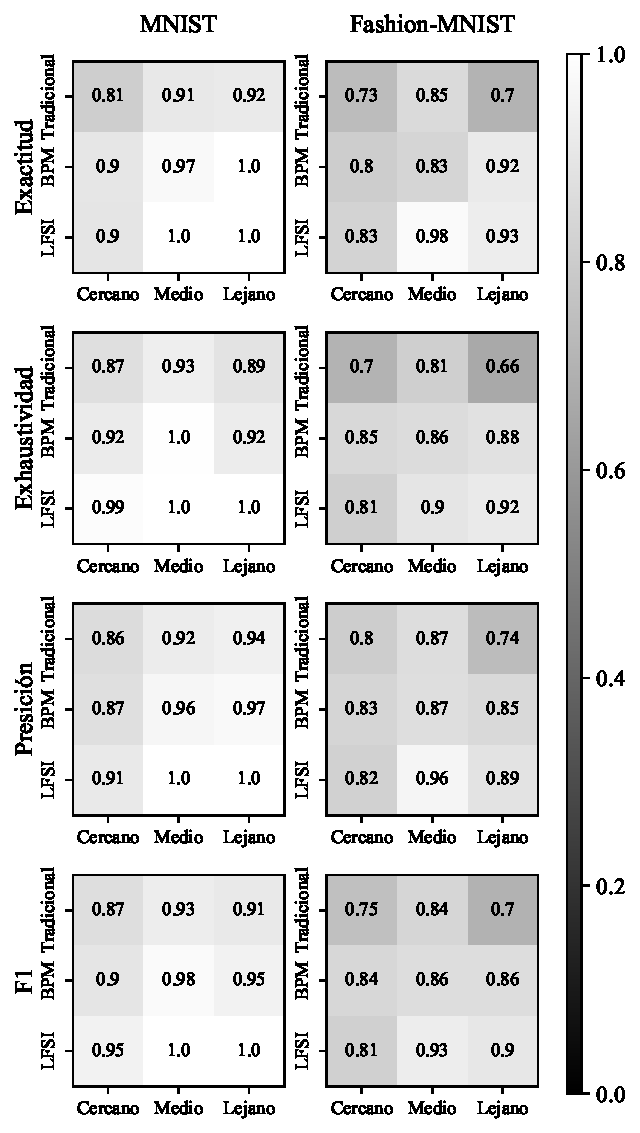
\includegraphics[height=0.8\textheight]{images/resultados/test_result_mobilnet.pdf}
    \label{fig:results_mob}
\end{figure}


\begin{figure}[!h]
    \centering
    \caption{Resultados en la métrica de exactitud, precisión, exhaustividad y F1 para evaluar la clasificación de medidas cuadráticas codificadas simuladas sobre el campo cercano, medio y lejano. Se muestra la comparación de la clasificación Tradicional, el uso del propagador inverso propuesto (BPM) y el método de inicialización aprendida (LFSI) usando la arquitectura InveptionV3, sobre la división de prueba de los conjuntos de datos MNIST y Fashion-MNIST.}
    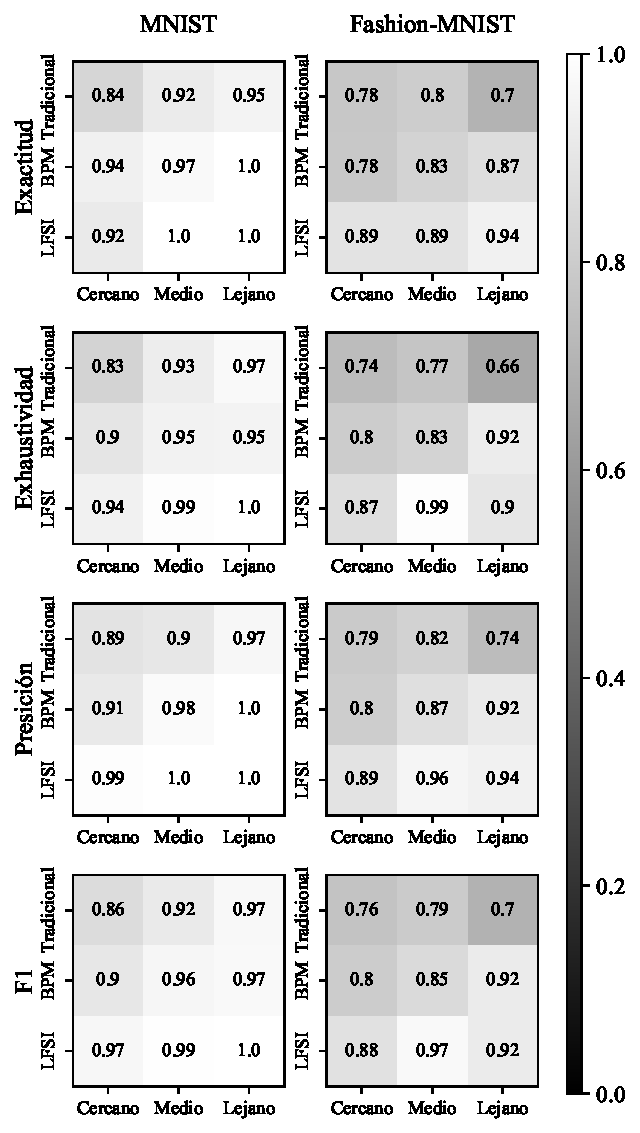
\includegraphics[height=0.8\textheight]{images/resultados/test_result_inception.pdf}
    \label{fig:results_inc}
\end{figure}

\begin{figure}[!h]
    \centering
    \caption{Resultados en la métrica de exactitud, precisión, exhaustividad y F1 para evaluar la clasificación de medidas cuadráticas codificadas simuladas sobre el campo cercano, medio y lejano. Se muestra la comparación de la clasificación Tradicional, el uso del propagador inverso propuesto (BPM) y el método de inicialización aprendida (LFSI) usando la arquitectura Xception, sobre la división de prueba de los conjuntos de datos MNIST y Fashion-MNIST.}
    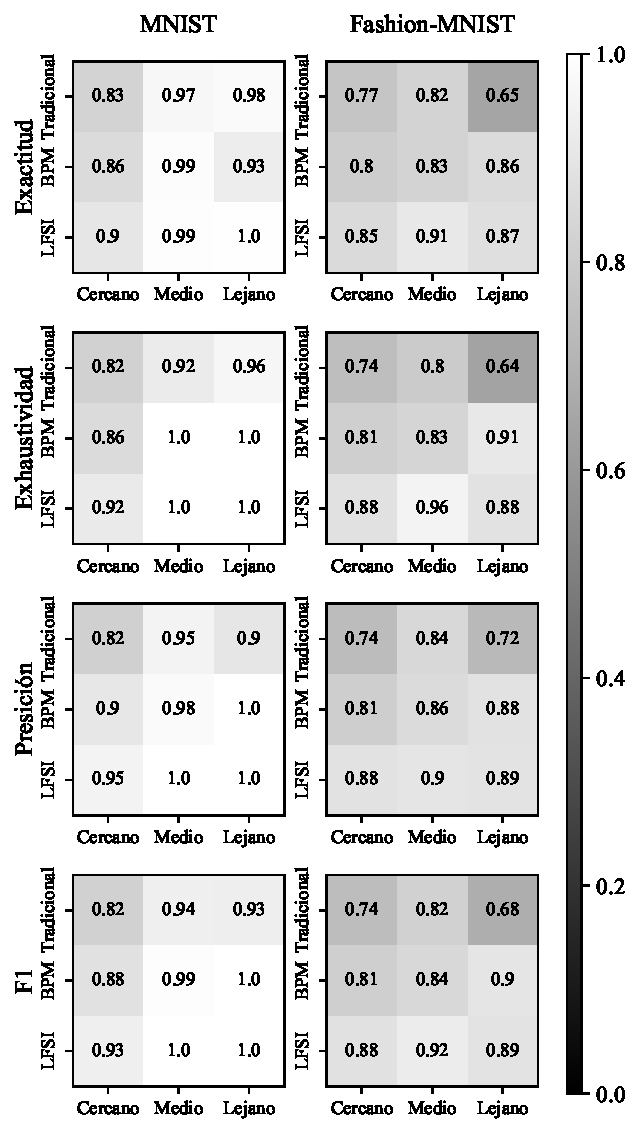
\includegraphics[height=0.8\textheight]{images/resultados/test_result_xception.pdf}
    \label{fig:results_xce}
\end{figure}
